\documentclass[a4paper,10pt]{article}
\usepackage[utf8x]{inputenc}
\usepackage{cite}
\usepackage{graphicx}
\usepackage[active,tightpage]{pstricks}
\usepackage{epstopdf}
\usepackage{float}
\usepackage[margin=1in, a4paper]{geometry}
\graphicspath{{Diagrams/}}

%opening
\title{A Workbench for Simple Asynchronous Circuit Simulation}
\author{Ran Ju}
\date{12 May 2012}

\begin{document}

\maketitle

\begin{abstract}

\end{abstract}
\tableofcontents
\section{Introduction}
Logic circuits are ubiquitous nowadays.  Most of them are based on the conventional design --- synchronous design\cite[Page 3]{bible}.  In a synchronous design, the state holding components (flip-flops and registers, as opposed to logic components or gates, which are stateless) are periodically enabled and disabled by a shared global clock signal, to store and relay their logic value, with logic gates interconnecting them.  Such a circuit is also referred to as a ``sequential circuit'', as opposed to combinational circuits (consisting of logic gates only, so are stateless).  Figure \ref{fig:in1} illustrates a common model of sequential circuits.

\begin{figure}[H] \label{fig:in1}
\centering
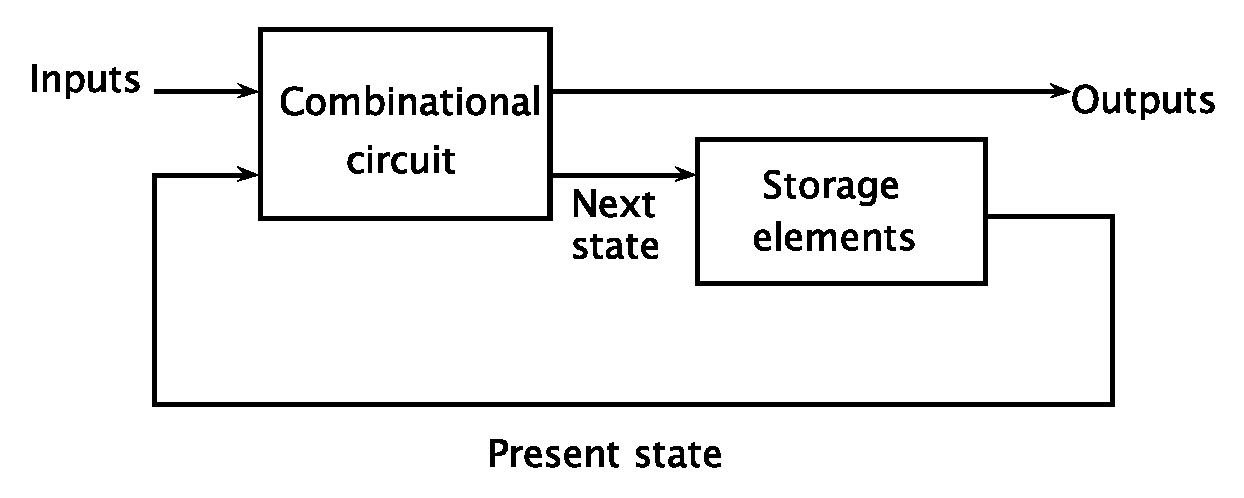
\includegraphics[scale=.5]{combination_circuit.eps}
\caption{Block Diagram of a Sequential Circuit\cite[Page 226]{basic}}\label{fig:in2}
\end{figure}

This design has the advantage that it is relatively easy to implement and verify the correctness of a circuit.  However, the such circuits are usually more power consuming, due to the fact that all storage elements are enabled and disabled constantly regardless where they will be set or not.  Another drawback is that the circuit is subject to the global worst-case latency.  If a number of circuits (as in Figure \ref{fig:in1}) are connected, then proper delays have to be introduced between them to ensure that they stay in sync.  

Asynchronous circuits, on the other hand, does not employ a global clock signal, in other words, no common and discreet time.  Instead, the circuits use handshaking between their components to perform the necessary synchronization, communication, and sequencing of operations\cite[Page 3]{bible}.  

The advantages of asynchronous circuits are almost what their synchronous counterparts lack.  Because there is no global clock signal, there is almost zero standby power consumption.  This makes them particularly attractive to mobile device manufacturers\cite[Chapter 7]{jones}.  All components operate at their own speed and with proper synchronization, each component can achieve its highest operating speed\cite[Page 3]{bible}.  

However, asynchronous circuits suffer from the same timing problem as synchronous ones.  Delays on wires and gates can signals may not propagate through the circuit as expected.  The following chapters give a brief introduction to asynchronous designs and simulation.

\subsection{Asynchronous Designs}!
A typical model of asynchronous circuits is in Figure \ref{fig:in2}.

\begin{figure}[H] 
\centering
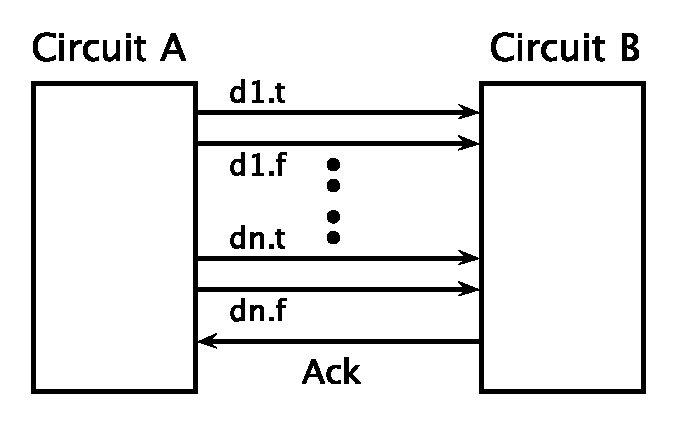
\includegraphics[scale=.7]{asynchronous_model.eps}
\caption{Dual-rail asynchronous circuit model\cite[Page 13]{bible}} \label{fig:in2}
\end{figure}

There are $n$ pairs of wires (dual rail), each pairing representing one of 3 states of the input signal: one(di.t=1, di.f=0), zero(di.t=0, di.f=1) and empty(di.t=0, di.f=0). The state (di.t=1, di.f=1) is not allowed.  The circuit implements a 4-phase hand-shaking protocol.  Initially, circuit A has all outputs empty, and acknowledgment(ack) is 0.  When circuit A observes acknowledgment signal changing from 1 to 0, it starts changing its outputs to valid values.  After all outputs are valid, circuit B is allowed to set ack to 0.  After observing 0 on ack, circuit changes outputs to empty.  The cycle is illustrated in \ref{fig:in3}

\begin{figure}[H] 
\centering
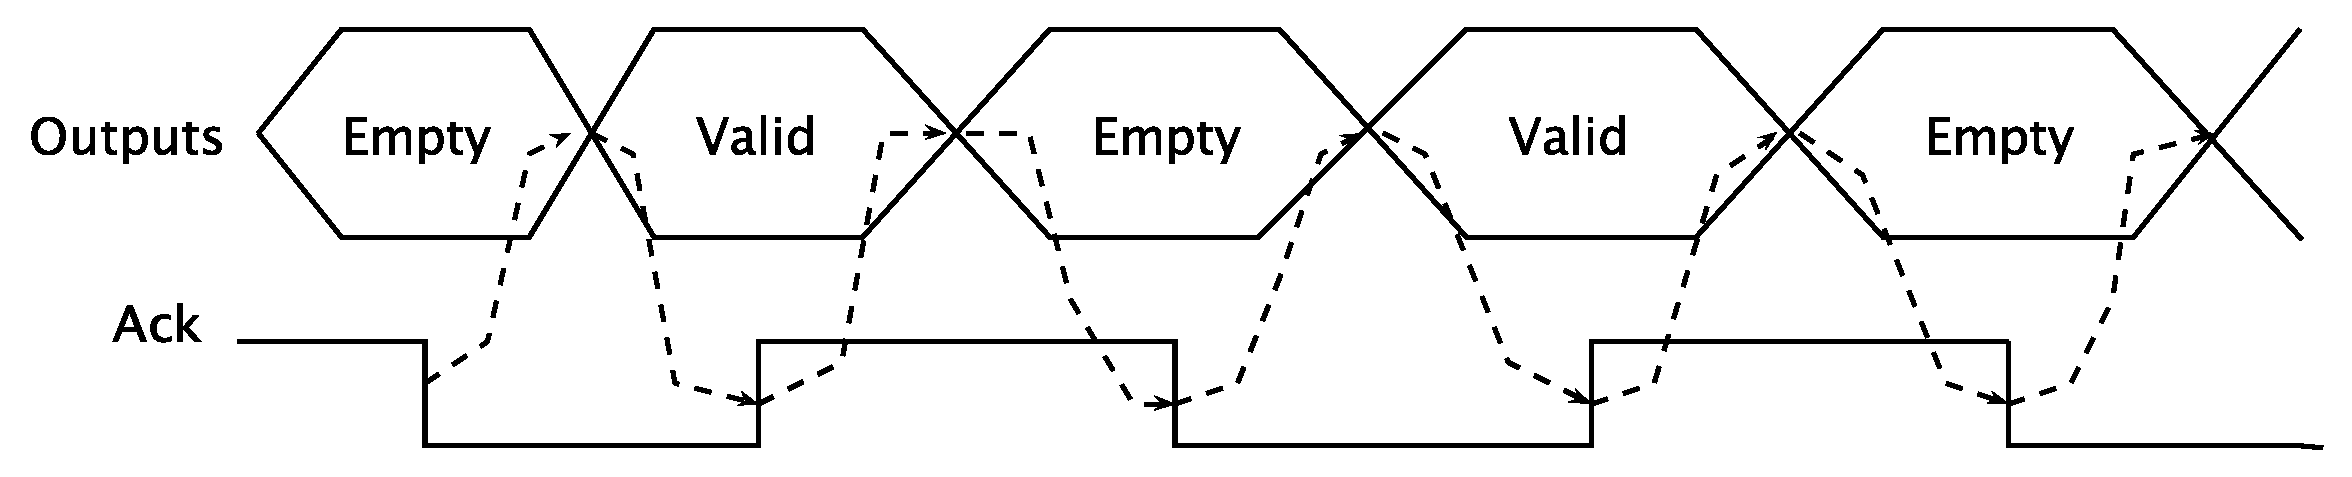
\includegraphics[scale=.3]{4phase_dual_rail.eps}
\caption{4-phase dual-rail handshake\cite[Page 13]{bible}} \label{fig:in3}
\end{figure}





\section{What}

\bibliographystyle{plain}
\bibliography{Report}
\end{document}

